\documentclass[UTF-8]{ctexart} 
\usepackage[a4paper,left=2cm,right=2cm,top=2.5cm,bottom=2.5cm]{geometry}
\usepackage{amsmath,bm,amssymb}
\usepackage[version=4]{mhchem}
\usepackage{siunitx}
\usepackage{physics}
\usepackage{lmodern}
\usepackage{tikz}
\usepackage{cutwin}
\usepackage{fancyhdr}
\usepackage{caption}
\usepackage{enumitem}
\usepackage{upgreek}
\usepackage{circuitikz}
\usepackage{mathrsfs}
\usetikzlibrary{snakes,fadings,patterns,patterns.meta}
\usetikzlibrary{decorations.markings}
\usetikzlibrary{decorations.pathmorphing}
\usetikzlibrary{shapes}
\usetikzlibrary{arrows.meta}
\usetikzlibrary{angles,quotes} 

\tikzfading[name=fade left, left color=transparent!30, right color=transparent!70]

\captionsetup{labelformat=empty}
%\renewcommand\thefigure{\theenumi}
\makeatletter
\renewcommand*\maketitle{
    \begin{center}
        \bfseries
        {\Large \@title \par}
        \vskip 1em
        {\global\let\author\@empty}
        {\global\let\date\@empty}
    \end{center}
  \setcounter{footnote}{0}
}
\newcommand{\mlabel}[2]{#2\def\@currentlabel{#2}\label{#1}}
\newcommand{\cube}[5]{
    \pgfmathsetmacro{\cubex}{#2}
    \pgfmathsetmacro{\cubey}{#3}
    \pgfmathsetmacro{\cubez}{#4}
    \filldraw[#5!50,join=round] #1 -- ++(-\cubex,0,0) -- ++(0,-\cubey,0) -- ++(\cubex,0,0) -- cycle;
    \filldraw[#5,join=round] #1 -- ++(0,0,-\cubez) -- ++(0,-\cubey,0) -- ++(0,0,\cubez) -- cycle;
    \filldraw[#5!80,join=round] #1 -- ++(-\cubex,0,0) -- ++(0,0,-\cubez) -- ++(\cubex,0,0) -- cycle;
}
\renewcommand\theenumi{S-\arabic{enumi}}
\renewcommand\labelenumi{\theenumi}
\sisetup{inter-unit-product = \ensuremath { { } \cdot { } } }
\newcommand{\csi}[2]{ \SI{#1}{#2}}
\newcommand{\cang}[1]{ \ang{#1}}
\newcommand*{\dif}{\mathop{}\!\mathrm{d}}
\newcommand{\lbd}[3]{\(\lambda_{#3}=\csi{#1}{#2}\)}
\newcommand{\ri}[2]{\(n_{#2}={#1}\)}
\newcommand{\tangle}[1]{\(\theta=\ang{#1}\)}
\makeatother

\pagestyle{fancy}
\fancyhf{}
\cfoot{\thepage}
\renewcommand\headrulewidth{0pt}
\title{第11章\ 光学}
\author{叶旺全\\大学物理教研室}

\begin{document} 
\maketitle
\begin{enumerate}
    %\item[\mlabel{itm:a}{5-6}] 自定义label引用参考
    \item[11-11] 在双缝干涉实验中,用波长\lbd{546.1}{\nm}{}的单色光照射,双缝与屏的距离\(d^\prime=\csi{300}{\mm}\)。现测得中央明纹两侧
        的两个第五级明纹的间距为\csi{12.2}{\mm},求双缝间的距离。
    \item[\mlabel{itm:14}{11-14}] 如图所示,由点\(S\)发出的\lbd{600}{\nm}{}的单色光,自空气入折射率\ri{1.23}{}的透明物质,再射入空气。若透明物质的
        厚度\(d=\csi{1.0}{\cm}\),入射角\tangle{30},且\(SA=BC=\csi{5.0}{\cm}\),问:(1)折射角\(\theta_1\)为多少?(2)此单色光再这层透明物质
        里的频率、速度和波长各为多少?(3)\(S\)到\(C\)的几何路程为多少?光程又为多少?
        \begin{figure}[htb]
            \centering
            \begin{minipage}[b]{0.4\textwidth}
                \centering
                \begin{tikzpicture}[>=stealth,decoration={markings,mark=at position 0.4 with {\arrow{>}}}]
                    \draw (-2,0) rectangle (2,-1);
                    \draw[dashed] (0,-1.5) coordinate (D) -- (0,1) coordinate (E);
                    \draw[postaction={decorate},cyan,thick] (120:2) coordinate (S) -- (0,0) coordinate (A) node[black,above right]{\(A\)}; 
                    \draw[fill] (120:2) node[left]{\(S\)} circle (1pt);
                    \pgfmathparse{asin(sin(30)/1.23)}
                    \let \rang \pgfmathresult
                    \draw[cyan,thick] (0,0) -- ({1*tan{\rang}},-1) coordinate["\(B\)" {below,black,xshift=-2mm}] (B);
                    \draw[postaction={decorate},cyan,thick] (B) -- ++(-60:2) coordinate["\(C\)" {right,black}] (C);
                    \draw[fill] (C) circle (1pt);
                    \pic[draw,thin,"\(\theta\)",angle radius=3mm,angle eccentricity=1.5]{angle=E--A--S};
                    \pic[draw,thin,"\(\theta_1\)" left,angle radius=3mm]{angle=D--A--B};
                    \node[right] at (-2,-0.5){\(n\)};
                    \draw[<->] (1.5,0) -- node[right]{\(d\)} (1.5,-1);
                    \node[above right] at (-2,0) {空气};
                    \node[below right] at (-2,-1) {空气};
                \end{tikzpicture}
                \caption{\ref{itm:14} 题图}
            \end{minipage}
        \end{figure}
    \item[11-15] 一双缝装置的一个缝被折射率为\csi{1.40}{}的薄玻璃片所遮盖,另一个缝被折射率为\csi{1.70}{}的薄玻璃片所遮盖。在玻璃片插入以后,屏上
        原来的中央极大所在点变为第五级明纹。假定\lbd{480}{\nm}{},且两玻璃片厚度均为\(d\),求厚度\(d\)。
    \item[11-16] 白光垂直照射到空气中一厚度为\csi{380}{\nm}的肥皂膜上。设肥皂膜的折射率为\csi{1.32}{}。试问该膜的正面呈现什么颜色?背面呈现什么颜色?
    \item[11-17] 折射率\ri{1.52}{3}的照相机镜头表面涂油一层折射率\ri{1.39}{2}的\,\ce{MgF2}增透膜,若此膜仅适用于\lbd{550}{\nm}{}的光,则此膜的最小厚度为多少?
    \item[\mlabel{itm:20}{11-20}] 如图所示,将符合标准的轴承钢珠a、b和待测钢珠c一起放在两块平板玻璃之间,若入射光的波长\lbd{580}{\nm}{},
        问钢珠c的直径比标准小多少?如果距离\(d\)不同,那么对检测结果有何影响?
        \begin{figure}[htb]
            \centering
            \begin{minipage}[b]{0.4\textwidth}
                \centering
                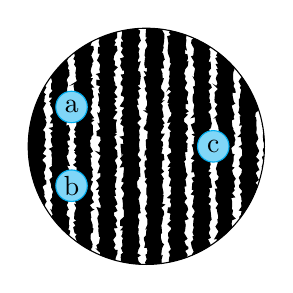
\begin{tikzpicture}[>=stealth,decoration={random steps,segment length=1pt,amplitude=0.8pt}]
                    \clip[draw] (0,0) circle(1.5);
                    \foreach \x in {-1.8,-1.5,...,1.8}
                        \draw[fill=black,decorate] (\x,1.8) rectangle ++(0.2,-3.6);
                    \draw[draw=cyan,fill=cyan!50] (-0.95,0.5) node{a} circle (0.2);
                    \draw[draw=cyan,fill=cyan!50] (-0.95,-0.5) node{b} circle (0.2);
                    \draw[draw=cyan,fill=cyan!50] (0.85,0) node{c} circle (0.2);
                \end{tikzpicture}
                \caption{\ref{itm:20} 题图}
            \end{minipage}
        \end{figure}
    \item[11-21] 折射率为\csi{1.60}{}的两块标准平面玻璃板之间形成一个劈形膜(劈尖角\(\theta\)很小)。用波长\lbd{600}{\nm}{}的单色光垂直入射,产生等厚干涉
        条纹。假如在劈形膜内充满\ri{1.40}{}的液体时的相邻明纹间距比劈形膜内是空气时的间距缩小\(\Delta I=\csi{0.50}{\mm}\),那么劈尖角\(\theta\)应是多少?
    \item[11-24] 在牛顿环实验中,当透镜与玻璃间充满某种液体时,第10个亮环的直径由\csi{1.40e-2}{\m}变为\csi{1.27e-2}{\m},试求这种液体的折射率。
    \item[\mlabel{itm:25}{11-25}] 如图所示,折射率\ri{1.2}{2}的油滴落在\ri{1.50}{3}的平板玻璃上,形成一上表面近似于球面的油膜,测得油膜中心最高处的
        高度\(d_m=\csi{1.1}{\um}\),用\lbd{600}{\nm}{}的单色光垂直照射油膜。问:(1)油膜周边是暗环还是明环?(2)整个油膜可看到几个完整暗环?
        

    \item[11-26] 某人用迈克耳孙干涉仪测量一光波的波长。在可动反射镜M移动\csi{0.310}{\mm}的过程中,观察到干涉条纹移动了1100条,求该光波的波长。
    \item[\mlabel{itm:27}{11-27}] 如图所示,狭缝宽度\(b=\csi{0.60}{mm}\),透镜焦距\(f=\csi{0.40}{\m}\),一个与狭缝平行的屏放置在透镜的焦平面处。若以单色
        平行光垂直照射狭缝,则在屏上离点\(O\)为\(x=\csi{1.4}{\mm}\)的点\(P\)看到衍射明条纹。试求:(1)该入射光的波长;(2)点\(P\)条纹的级数;(3)从点
        \(P\)处来看,对该光波而言,狭缝处的波阵面可分成的半波带数目。
        \begin{figure}[htb]
            \centering
            \begin{minipage}[b]{0.4\textwidth}
                \centering
                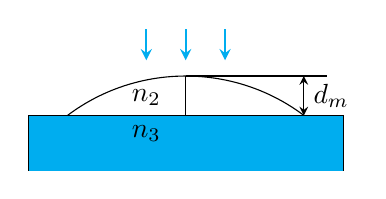
\begin{tikzpicture}[>=stealth]
                    \draw[yshift=-2cm] (45:2.5) arc (45:135:2.5);
                    \draw[fill=cyan] (-2,-0.7) -- (-2,0) -- (2,0) -- (2,-0.7);
                    \foreach \x in {-0.5,0,0.5}
                        \draw[thick,cyan,<-] (\x,0.7) -- ++(0,0.4);
                    \draw (0,0.5) -- ++(1.8,0);
                    \draw[<->] (1.5,0) -- node[right]{\(d_m\)} ++(0,0.5);
                    \draw[very thin] (0,0) -- (0,0.5);
                    \node[above] at (-0.5,0){\(n_2\)};
                    \node[below] at (-0.5,0){\(n_3\)};
                \end{tikzpicture}
                \caption{\ref{itm:25} 题图}
            \end{minipage}
            \begin{minipage}[b]{0.4\textwidth}
                \centering
                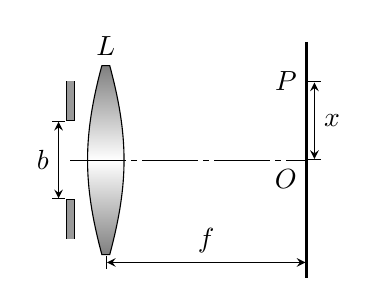
\begin{tikzpicture}[>=stealth]
                    \draw[fill=gray!80] (-0.05,1) -- ++(0,-0.5) -- ++(0.1,0) -- ++(0,0.5);
                    \draw[fill=gray!80] (-0.05,-1) -- ++(0,0.5) -- ++(0.1,0) -- ++(0,-0.5);
                    \draw[top color=gray,bottom color = gray,middle color = white,draw = black] (0.4,1.2) -- node[above]{\(L\)} (0.5,1.2) to [bend left=15] (0.5,-1.2) -- (0.4,-1.2) to [bend left=15] (0.4,1.2);
                    \draw[very thick] (3,1.5) -- (3,-1.5);
                    \draw[|<->|] (-0.15,0.5) -- node[left]{\(b\)} (-0.15,-0.5);
                    \draw[dash pattern={on 20pt off 2pt on 2pt off 2pt}] (0,0) -- (3,0);
                    \draw[|<->|] (0.45,-1.3) -- node[above]{\(f\)} (3,-1.3);
                    \draw[|<->|] (3.1,0) -- node[right]{\(x\)} (3.1,1) node[left=1mm]{\(P\)};
                    \node[below left] at (3,0) {\(O\)};
                \end{tikzpicture}
                \caption{\ref{itm:27} 题图}
            \end{minipage}
        \end{figure}
    \item[11-29] 一单色平行光垂直照射于一单缝,若其第三级明纹位置正好和波长为\csi{600}{\nm}的单色光入射时的第二级明纹位置一样,则求前一种单色光的波长。
    \item[11-30] 已知单缝宽度\(b=\csi{1.0e-4}{\m}\)透镜焦距\(f=\csi{0.50}{\m}\),用\lbd{400}{\nm}{1}和\lbd{760}{\nm}{2}的单色平行光分别垂直照射,
        求这两种光的第一级明纹离屏中心的距离,以及这两条明纹之间的距离。若用每厘米刻有1000条刻线的光栅代替这个单缝,则这两种单色光的第一级明纹分别
        距屏中心多远?这两条明纹之间的距离又是多少?
    \item[11-32] 老鹰眼睛的瞳孔直径约为\csi{6}{\mm},问其最高飞翔多高时可看清地面上身长为\csi{5}{\cm}的小鼠?设光在空气中的波长为\csi{600}{\nm}。
    \item[11-33] 一束平行光垂直入射到某个光栅上,该光束有两种波长的光,\lbd{440}{\nm}{1}和\lbd{660}{\nm}{2}。实验发现,两种波长的谱线(不计中央明纹)
        第二次重合于衍射角\(\varphi=\ang{60}\)的方向上,求此光栅的光栅常量。
    \item[11-34] 用一毫米内有500条刻痕的平面透射光栅观察钠光谱(\lbd{589}{\nm}{}),设透镜焦距\(f=\csi{1.00}{\m}\)。问(1)光栅垂直入射时,最多能看到
        第几级光谱?*\negthinspace(2)光线以入射角\cang{30}入射时,最多能看到第几级光谱?(3)若用白光垂直照射光栅,第一级光谱的线宽度是多少。
    \item[11-37] 今测得从一池静水的表面反射出来的太阳光是线偏振光,问此时太阳处于地平线上的多大仰角处(水的折射率为1.33)?
    \item[11-38] 使自然光通过两个偏振化方向相交\cang{60}的偏振片,透射光强为\(I_1\)。今在这两个偏振片之间插入另一偏振片,它的偏振化方向与前两个偏振片均
        成\cang{30}角,则透射光强为多少?
    \item[11-39] 一束光是自然光和平面线偏振光的混合,当它通过一个偏振片时,发现透射光的强度取决于偏振片的取向,其强度可以变化5倍。问入射光中两种光的
        强度各占总入射光强度的几分之几?
    \item 用很薄的云母片(\ri{1.58}{})覆盖在双缝实验中的一条缝上,这时屏幕上的零级明条纹移到原来的第七级明纹的位置上,如果入射光波长为\csi{550}{\nm},
        试问此云母片的厚度为多少?(假设光通过云母片时不考虑折射引起的光线偏折)
    \item \label{itm:s2} 设劳埃德镜的镜长有\csi{5.0}{\cm},幕与镜边缘的距离为\csi{3.0}{\m},缝光源离镜面高度为\csi{0.5}{\mm},水平距离\csi{2.0}{\cm},
        光波长为\csi{589.3}{\nm}。求幕上条纹的间距。幕上能出现几条干涉条纹?
        \begin{figure}[htb]
            \centering
            \begin{minipage}[b]{0.8\textwidth}
                \centering
                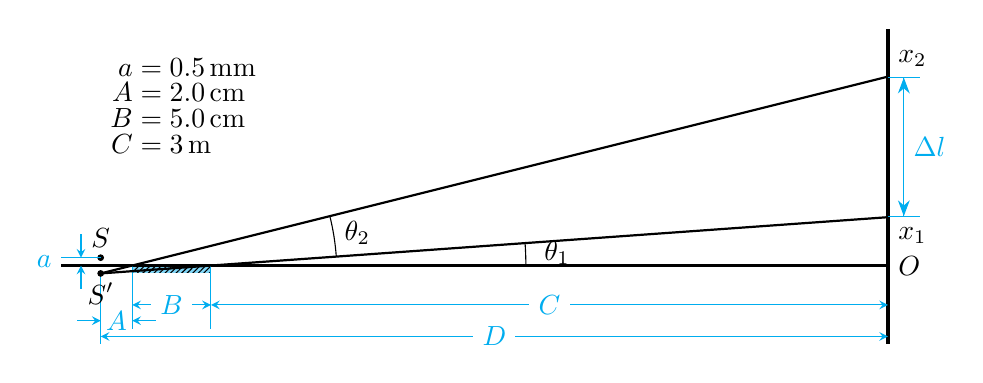
\begin{tikzpicture}[>=stealth]
                    \draw[very thick] (10,3) -- (10,-1);
                    \draw[fill=cyan!50,draw=white] (0.4,0) rectangle ++(1,-0.1);
                    \draw[pattern={Lines[angle=45,distance={2pt/sqrt(2)}]},draw=white] (0.4,0) rectangle ++(1,-0.1);
                    \draw[thick] (-0.5,0) -- (1.4,0) coordinate (B) -- (10,0) coordinate["\(O\)" right] (O);
                    \draw[fill] (0,0.1) node[above]{\(S\)} circle (1pt);
                    \draw[cyan] (0,-0.1) -- (0,-1) (0.4,0) -- (0.4,-0.8) (1.4,0) -- (1.4,-0.8);
                    \draw[fill] (0,-0.1) coordinate (S) node[below]{\(S^\prime\)} circle (1pt);
                    \draw[thick] (S) -- ++(10,2.5) coordinate["\(x_2\)" above right] (x2);
                    \draw[thick] (S) -- ++(10,{10/14}) coordinate["\(x_1\)" below right] (x1);
                    \draw[cyan,arrows={Bar[width=4mm] Stealth[length=2mm] - Stealth[length=2mm] Bar[width=4mm]}] ($(x1)+(0.2,0)$) -- node[right]{\(\Delta l\)} ($(x2)+(0.2,0)$);
                    \draw[cyan,<->] (0,-0.9) -- node[fill=white]{\(D\)} (10,-0.9);
                    \draw[cyan,<->] (0.4,-0.5) -- node[fill=white]{\(B\)} (1.4,-0.5);
                    \draw[cyan,<->] (1.4,-0.5) -- node[fill=white]{\(C\)} (10,-0.5);
                    \draw[cyan,<-] (0,-0.7) -- (-0.3,-0.7);
                    \draw[cyan,<-] (0.4,-0.7) -- (0.7,-0.7);
                    \draw[cyan,<-] (-0.25,0.1) -- (-0.25,0.4);
                    \draw[cyan,<-] (-0.25,0) -- (-0.25,-0.3);
                    \node[cyan,left] at (-0.5,0.05) {\(a\)};
                    \node[cyan] at (0.2,-0.7) {\(A\)};
                    \draw[cyan] (0,0.1) -- (-0.5,0.1);
                    \pic[draw,"\(\theta_2\)",angle radius=3cm,angle eccentricity=1.1] {angle=x1--S--x2};
                    \pic[draw,"\(\theta_1\)",angle radius=4cm,angle eccentricity=1.1] {angle=O--B--x1};
                    \node[right] at (0,2) {
                        $\begin{aligned}
                        a&=\csi{0.5}{\mm}\\[-2mm]
                        A&=\csi{2.0}{\cm}\\[-2mm]
                        B&=\csi{5.0}{\cm}\\[-2mm]
                        C&=\csi{3}{\m}
                     \end{aligned}$};
                \end{tikzpicture}
                \caption{\ref{itm:s2} 题图}
            \end{minipage}
        \end{figure}
    \item 一平面单色光波垂直照射在厚度均匀的薄油膜上,油膜覆盖在玻璃板上。所用单色光的波长可以连续变化,观察到\csi{500}{\nm}与\csi{700}{\nm}这两个
        波长的光在反射中消失。油的折射率为\csi{1.30}{},玻璃的折射率为\csi{1.50}{},试求油膜的最小厚度。
    \item \label{itm:s4} 如图所示,G\(_1\)和G\(_2\)是两块块规(块规是两个端面经过磨平抛光,达到相互平行的钢质长方体),G\(_1\)的长度是标准的,G\(_2\)是
        同规格待校准的复制品(两者的长度差在图中是夸大的),G\(_1\)和G\(_2\)放置在平台上,用一块样板平玻璃T压住。(1)设垂直入射光的波长为\csi{589.3}{\nm},
        G\(_1\)和G\(_2\)相隔\(l=\csi{5}{\cm}\),T与G\(_1\)以及T与G\(_2\)间的干涉条纹的间隔都是\csi{0.5}{\mm}。试求G\(_1\)与G\(_2\)的长度差;
        (2)如何判断G\(_1\)、G\(_2\)哪一块比较长一些?(3)如果T与G\(_1\)间的干涉条纹的间距是\csi{0.5}{\mm},而T与G\(_2\)间的干涉条纹的间距是\csi{0.3}{\mm},
        则说明了什么问题?
        \begin{figure}[htb]
            \centering
            \begin{minipage}[b]{0.4\textwidth}
                \centering
                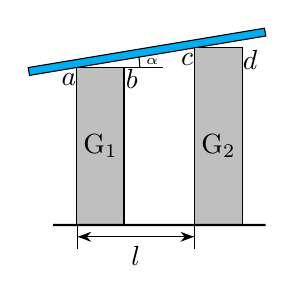
\begin{tikzpicture}[>=stealth]
                    \coordinate (A) at (0,0);
                    \coordinate (B) at (3,0.5);
                    \coordinate (a) at ($(A)!0.2!(B)$);
                    \coordinate (c) at ($(A)!0.7!(B)$);
                    \draw[fill=cyan,draw=black] (A) -- (B) -- ([turn]90:0.1) -- ++($(A)-(B)$) -- cycle;
                    \draw[fill=lightgray,draw=black] (a) rectangle ++(0.6,-2);
                    \draw[fill=lightgray,draw=black] let \p1=(a),\p2=(c) in 
                         (c) rectangle ++ (0.6,{-(2cm+\y2-\y1)}) coordinate (c2);
                    \draw[thick] ($(a)+(-0.3,-2)$) -- ($(c2)+(0.3,0)$);
                    \draw[thin] (a) -- ++(1.1,0) coordinate (b);
                    \pic[draw,"\tiny \(\alpha\)",angle radius=0.8cm,angle eccentricity=1.2] {angle=b--a--c};
                    \node[xshift=-1mm,yshift=-1.5mm] at (a) {\(a\)};
                    \node[xshift=1mm,yshift=-1.5mm] at ($(a)+(0.6,0)$) {\(b\)};
                    \node[xshift=-1mm,yshift=-1.5mm] at (c) {\(c\)};
                    \node[xshift=1mm,yshift=-1.5mm] at ($(c)+(0.6,0)$) {\(d\)};
                    \draw[arrows={Bar[width=3mm] Stealth[]-Stealth[] Bar[width=3mm]}] let \p1=(a),\p2=(c) in 
                        ($(a)+(0,-2.15)$) -- node[below]{\(l\)} ++(\x2-\x1,0);
                    \node at ($(a)+(0.3,-1)$){G\(_1\)};
                    \path let \p1=(a),\p2=(c) in node at ($(c)+(0.3,\y1-\y2-1cm)$){G\(_2\)};
                \end{tikzpicture}
                \caption{\ref{itm:s4} 题图}
            \end{minipage}
        \end{figure}
    \item 一带有玻璃窗的密封气室,长度为\csi{5.0}{\cm},把它放在迈克耳孙干涉仪的一臂上。实验中用波长为\csi{589}{\nm}的光。现在用真空泵将气室中的空气
        缓慢地抽出来,在抽气的过程中观察到有51条条纹通过视场。根据这些数据,试求在\csi{1.013e5}{\Pa}下空气的折射率。
    \item 用波长为\lbd{400}{\nm}{1}和\lbd{700}{\nm}{2}的混合光垂直照射单缝,在衍射图样中,\(\lambda_1\)的第\(k_1\)级明纹中心位置恰与\(\lambda_2\)的
        第\(k_2\)级暗纹中心位置重合。求\(k_1\)和\(k_2\)。试问\(\lambda_1\)的暗纹中心位置能否与\(\lambda_2\)的暗纹中心位置重合。
    \item 已知地球到月球的距离是\csi{3.84e8}{\m},设来自月球的光的波长为\csi{600}{nm},若在地球上用物镜直径为\csi{1}{\m}的天文望远镜观察时,
        刚好将月球正面一环形山上的两点分辨开,则该两点的距离为多少?
    \item 波长\csi{600}{\nm}的单色光垂直入射在一光栅上。第二级明纹出现在\(\sin \theta = 0.20\) 处,且第四级缺级。试问:
        (1)光栅上相邻两缝的间距\(b+b^\prime\)有多大?(2)光栅上狭缝可能的最小宽度\(b\)有多大?(3)按上述选定的\(b\)、\(b^\prime\)值,
        试问在光屏上可能观察到的全部明条纹数是多少?
    \item 一厚度为\csi{10}{\um}的方解石晶片,其光轴平行于表面,放置在两正交偏振片之间,晶片的光轴与第一偏振片的偏振化方向夹角为\cang{45},
        若要使波长为\csi{600}{\nm}的光通过上述系统后呈现极大,晶片的厚度至少需要磨去多少?
\end{enumerate}
\end{document} 